\chapter{Conclusion}\label{ch:conclusion}

	There is great motivation to combat HAIs not only for the patient's well being but also from fiscal perspective for the hospital. Estimates of the cost of these infections, suggest that the annual economic costs are \$6.7 billion per year in the United States \cite{martone1992incidence} and \pounds1.06 billion (approximately US \$1.7 billion) in the United Kingdom \cite{plowman2001rate}. 
    
    The literature review demonstrates that the area of indoor positioning is a highly promising field. Its use in the health care industry has been focused around positioning and process flows. However, this mobility data has the potential to be used in new and innovative ways such as the aim for this thesis.
    
    The preliminary software design of the PDR system has shown promising results. More experiments need to be conducted in order to come to a definite conclusion on the accuracy of the PDR algorithms used. 
	
	\section{Future Work} \label{sec:conclusion_future}
    
    	This progress report lays the foundation for the successful completion of the following areas of work. Figure \ref{fig:conclusion_ganttChart} graphically outlines the planned future activities.
        
        \begin{sidewaysfigure}
          \fbox{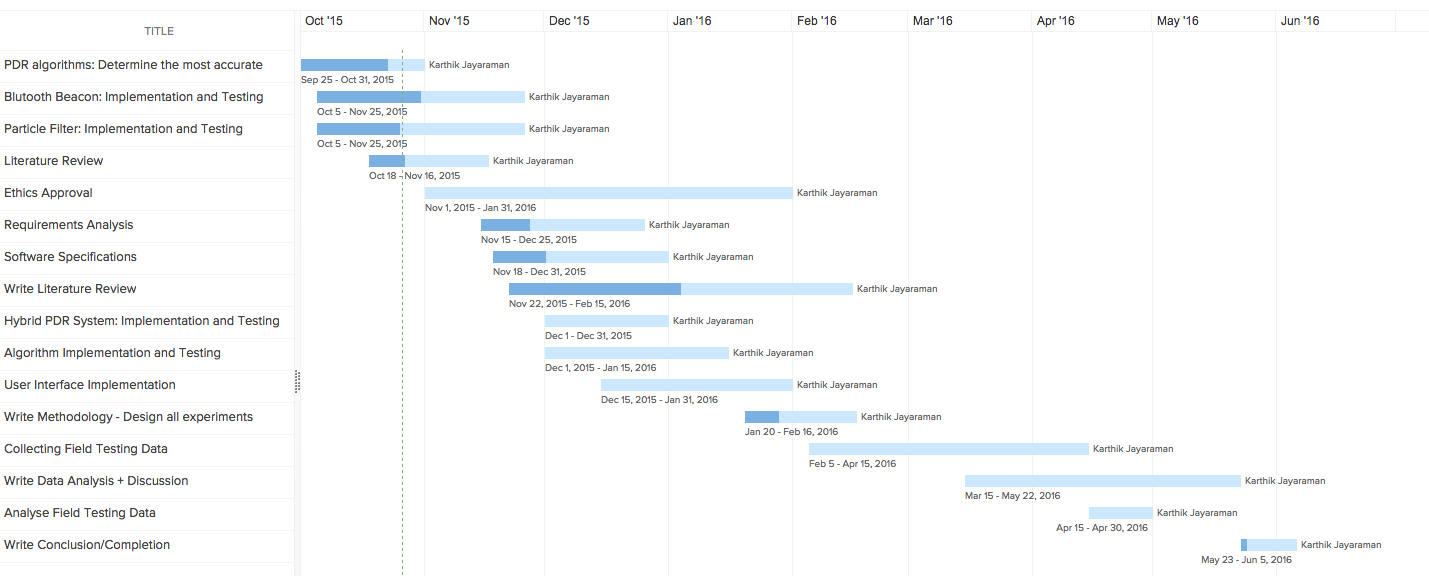
\includegraphics[width=\textwidth,scale=1.2]{planGantt}}
          \caption{Thesis Plan}
          \label{fig:conclusion_ganttChart}
        \end{sidewaysfigure}
    
    	\subsection{PDR Design}
        	The PDR system requires further analysis and testing to determine an accurate result. This involves further experimentation using various algorithms for step detection, step length calculation and heading estimation. 
            
            As with any PDR, drift is inevitable hence direct sensing technologies such as bluetooth beacons along with bayesian filters such as particle filters need to be incorporated to create a hybrid PDR system. This hybrid system will require further analysis and testing for verification and validation.
        
    % social network analysis        
        \subsection{SNA}
        	SNA implementation has not been conducted for Thesis A, hence it will form a core part of Thesis B activities. The main task include:
            \begin{enumerate}
				\item Further study of literature on SNA, specific to disease control and transmission
                \item Identifying algorithms that can be used to determine high risk areas
                \item Software implementation of the said algorithms
                \item Experimentation and testing to verify and validate the correctness of these algorithms
			\end{enumerate}
        
        % browser interface implementation
        \subsection{Software Design}
        	The final outcome for this thesis is to create a software package that incorporates both the PDR and SNA. A simple waterfall model approach was taken for the design of the PDR system. For future work, a more rigorous approach will be taken (possibly using the Agile Method) to identify and create the key components of the software system. 
        
        \subsection{Field Testing}
        	After successfully verifying and validating the software system, more specifically the PDR system. It is planned that these components be implemented in the hospital environment. The data collected from these tests can be used to verify the robustness of the software system as well as experimentations on SNA.
        